\documentclass[12pt,a4]{article}



\newcommand{\handoutdate}{Monday, 2019-10-21}
\newcommand{\firstduedate}{Monday, 2019-10-28}
\newcommand{\finalduedate}{Monday, 2019-11-04}




\usepackage{graphicx,amsmath,amssymb,amsthm, boxedminipage}



\usepackage{algorithm}
\usepackage{algpseudocode}


\newtheorem{theorem}{Theorem}%[section]
\newtheorem{proposition}[theorem]{Proposition}
\newtheorem{lemma}[theorem]{Lemma}
\newtheorem{corollary}[theorem]{Corollary}
\newtheorem{definition}[theorem]{Definition}



\newcommand{\scalar}[2]{\ensuremath{\langle #1, #2\rangle}}
\newcommand{\floor}[1]{\left\lfloor #1 \right\rfloor}
\newcommand{\ceil}[1]{\left\lceil #1 \right\rceil}
\newcommand{\norm}[1]{\|#1\|}
\newcommand{\pfrac}[2]{\left(\frac{#1}{#2}\right)}
\newcommand{\nth}[1]{#1\textsuperscript{th}}

% \newcommand{\nth}[1]{#1\textsuperscript{th}}
\newcommand{\E}{\mathop{\mathbb{E\/}}}
\newcommand{\N}{\mathbb{N}}

\newcommand{\R}{\mathbb{R}}

\newtheorem{exercise}[theorem]{Exercise}
\newtheorem{exerciseD}[theorem]{*Exercise}
\newtheorem{exerciseDD}[theorem]{**Exercise}

\let\oldexercise\exercise
\renewcommand{\exercise}{\oldexercise\normalfont}

\let\oldexerciseD\exerciseD
\renewcommand{\exerciseD}{\oldexerciseD\normalfont}

\let\oldexerciseDD\exerciseDD
\renewcommand{\exerciseDD}{\oldexerciseDD\normalfont}


 
\begin{document}

\date{}

\title{CS 217 -- Algorithm Design and Analysis \\ 
  \vspace{3mm}
{\large	Shanghai Jiaotong University, Fall 2019\\
}
}
\maketitle

\noindent
Handed out on \handoutdate{}\\
First submission and questions due on \firstduedate{}\\
You will receive feedback from the TA.\\
Final submission due on \finalduedate{}




\setcounter{section}{4}
\section{More on Network Flows}


\begin{exercise}
    Let $G = (V,c)$ be a flow network. Prove that flow is ``transitive'' in the following sense: if $r,s,t$ are vertices, 
    and there is an $r$--$s$-flow of value $k$ and an $s$--$t$-flow of value $k$, then there is an $r$--$t$-flow of 
    value $k$.
\end{exercise}

\subsection{Vertex Disjoint Paths}

Let $G$ be a directed graph. Two paths $p_1, p_2$ from $s$ to $t$ are called {\em vertex disjoint}
if they don't share any vertices except $s$ and $t$. 

\begin{theorem}[Menger's Theorem]
   Let $G$ be a graph and $s \ne t$ two vertices therein. Let $k \in \mathbf{N}_0$. 
   Then exactly one of the following is true:
   \begin{enumerate}
   \item There are $k$ vertex disjoint paths $p_1,\dots,p_k$ from $s$ to $t$; that is, no two $p_i$, $p_j$ share
   any vertex besides $s$ and $t$.
   \item There are vertices $v_1,\dots,v_k \in V \setminus \{s,t\}$ such that
   $G - \{v_1,\dots, v_k\}$ contains no $s$--$t$-path.
   \end{enumerate}
\end{theorem}

\begin{exercise}
   Prove Menger's Theorem. You have to prove two things: first, not both cases above can occur (this is rather easy);
   second, one of them must occur (this requires a tool from the lecture).
\end{exercise}
\begin{proof}
		$k$ is the value of the flow? 
\end{proof}


Let $V = \{0,1\}^n$. The $n$-dimensional Hamming cube $H_n$ is the graph $(V,E)$ where
$\{u,v\} \in E$ if $u,v$ differ in exactly one coordinate.
Define the $\nth{i}$ level of $H_n$ as 
\begin{align*}
  L_i := \{u \in V \ | \ \norm{u}_1 = i \} \ ,
\end{align*}
i.e., those vertices $u$ having exactly $i$ coordinates which are $1$.
\begin{center}
  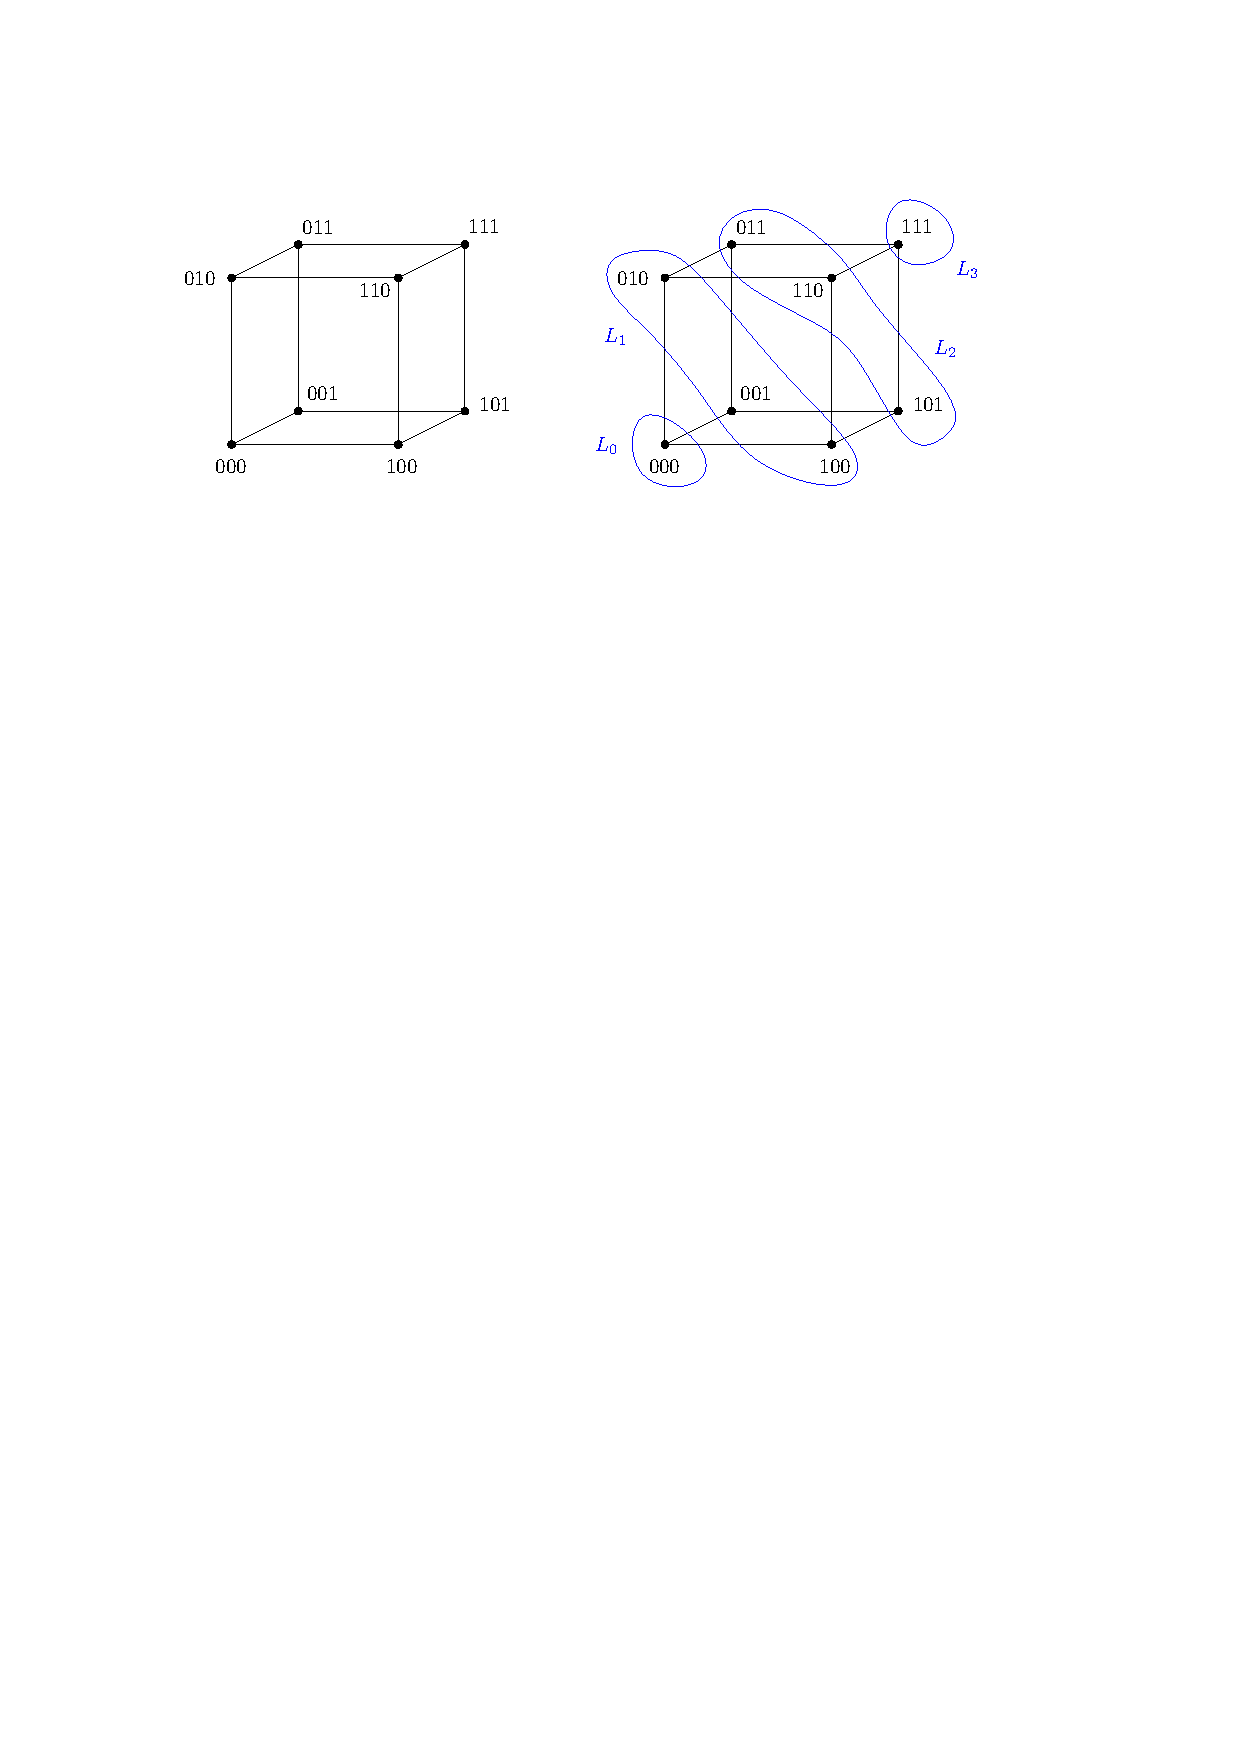
\includegraphics[width=0.8\textwidth]{figures/hamming-3-dim.pdf}\\
  {\small The $3$-dimensional Hamming cube and the four 
    sets $L_0$, $L_1$, $L_2$, $L_3$.}
\end{center}


\begin{exercise}[Matchings in $H_n$]
  Consider the induced bipartite subgraph $H_n[ L_i \cup L_{i+1}]$. This is 
  the graph on vertex set $L_i \cup L_{i+1}$ where two edges are connected
  by an edge if and only if they are connected in $H_n$.
  \medskip

  Show that for $i \leq n/2$ the graph $H_n[ L_i \cup L_{i+1}]$
  has a matching of size $|L_i| = {n \choose i}$.

\begin{center}
  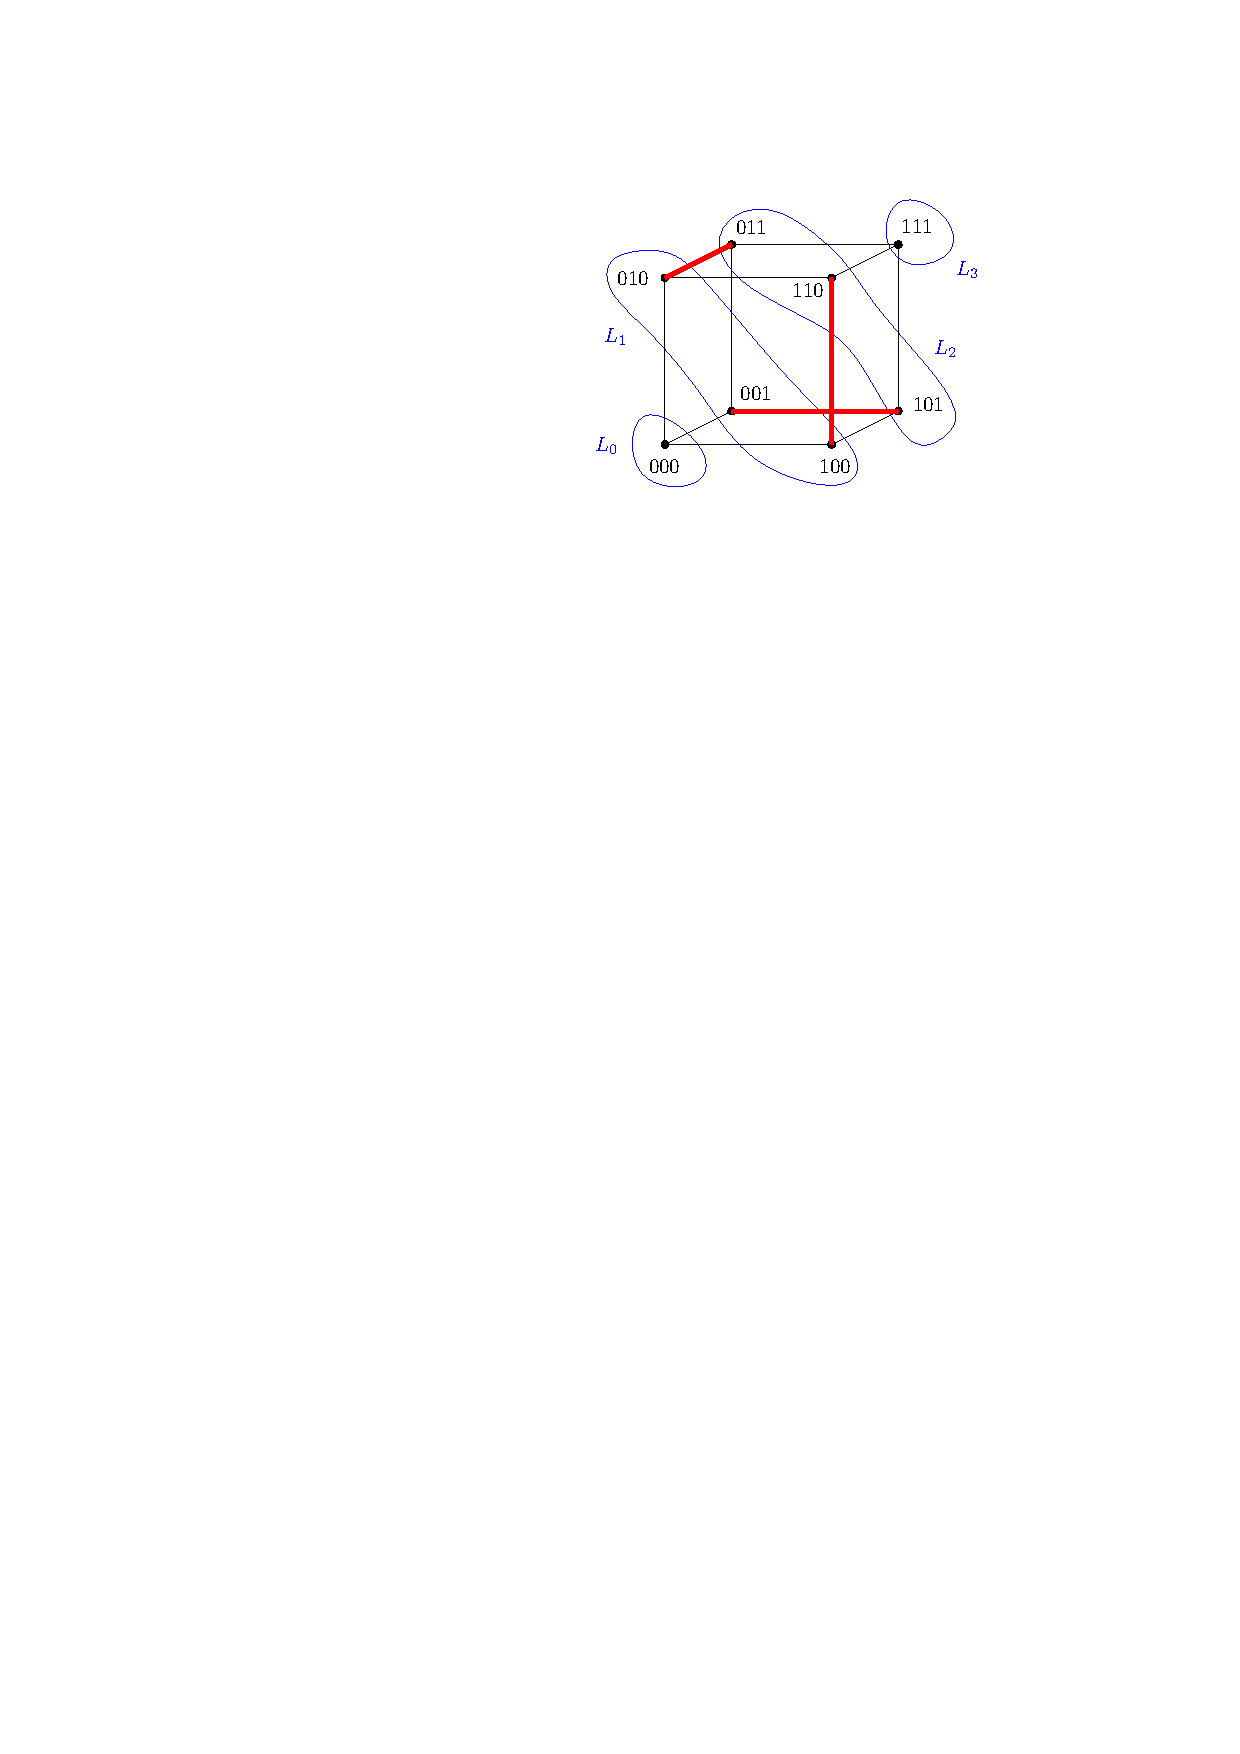
\includegraphics[width=0.4\textwidth]{figures/hamming-3-dim-matching.pdf}\\
  {\small A matching of size $3$ between $L_1$ and $L_2$.}
\end{center}
\label{exercise-matchings-in-H}
\end{exercise}
\begin{proof}
		Consider $v\in L_{i},$ we know there are $i$ bits to be  $1$. 
		Let $a_1,a_2,\ldots, a_i$ be that set of integers or indexes
		such that $\forall j \le i , v_{a_j}= 1$. That is, we use the indexes
		in which $v$ has value  $1$ to represent the vertex.

		Our goal is to construct a mapping $g: \{\N\times \ldots\times \N \}\to \N$, such
		that $\{ v_1,\ldots,v_{i}, g\left( v \right) \}= \left\{ \mathbf{v},g\left( v \right)  \right\} \in L_{i+1}$ , plus 
		$\forall u\neq v \in L_{i}$, we have 
		\[
				\{ u, g\left( u \right) \} \neq 
				\{ v, g\left( v \right) \} 
		.\] 	
		Let $n = \prod_{i=1}^{n} p_i ^{\alpha _i} $, consider the smallest prime 
		$p \not\in \{p_1,\ldots,p_n\} $, we construct the mapping $g$ 
		as following:
		\[
				g\left( u \right) = \left( p-1 \right) \left( 
				\sum_{j=1}^{i} u_{j}\right) \bmod n
		.\] 
		We assume $u$ maps to  $n$ if $g\left( u \right) = 0$. Now we prove
		this mapping is valid. Otherwise, there exists $u,v$ they have at least 1
		different elements, i.e. 
		\[ 
				i - \left|u \cap v\right| \ge 1. 
		\]
		Plus 
		$\{u,g\left( u \right) \} = \{v, g\left( v \right) \} $. We must have 
		\[
		\left| u\cap v \right| = i- 2
		.\] 
		Assume $u=\{ a_1,\ldots,a_{i-1}, g\left( v \right) \},v =\{ a_1,\ldots
		a_{i-1}, g\left( u \right) \} $. 
		Hence 
		\begin{align*}
				g\left( u \right)  =&\left( p-1 \right)  \left( \sum_{j=1}^{i-1} a_{i} + g\left( v \right) \right) \bmod n \\
				g\left( v \right)  =&  \left( p-1 \right) \left( \sum_{j=1}^{i-1} a_i + g\left( u \right)  \right)  \bmod n
		.\end{align*}
		Which leads that 
		\[
				p\left( g\left( u \right) -g\left( v \right)  \right) = 0 \pmod n 
		.\] 
		Hence 
		\[
				u = \{a_1, \ldots, a_{i-1}, g\left( v \right) \} =
				\{ a_1,\ldots,a_{i-1}, g\left( u \right) \} =
				v
		.\] 
		It contradicts with the assumption that $u\neq v$, thus the mapping 
		$g$ is a valid one. And $H_n\left[ L_i \cap L_{i+1} \right] $ has a 
		matching!
\end{proof}
\begin{exercise} 
  Let $H_n$ be the $n$-dimensional Hamming cube. For $i < n/2$ consider
  $L_i$ and $L_{n-i}$. Note that 
  $|L_i| = {n \choose i} = { n \choose n-i}  = L_{n-i}$, so the 
  $L_i$ and $L_{n-i}$ have the same size.   Show that there are ${n \choose i}$ paths $p_1,p_2,\dots,p_{ {n \choose i}}$
  in $H_n$ such that
  (i) each $p_i$ starts in $L_i$ and ends in $L_{n-i}$;
  (ii) two different paths $p_i,p_j$ do not share any vertices.
  \textbf{Hint 1.} Model this problem as a network flow with vertex capacities. What would 
  the maximum flow be in this network?
  \textbf{Hint 2.} It's not {\em that} easy. If you try to work from both sides towards
  the middle by combining matchings between levels, 
  you will certainly run into problems as how to glue things together in the middle.
  I have never seen any ``meet in the middle'' proof that works.
  \textbf{Hint 3.} There is a ``direct'' proof by induction that does not require anything
  about network flows.

\end{exercise}
\begin{proof}
		It is well known that $\binom{i}{n} \le\binom{i+1}{n} \le \ldots \le \binom{\frac{n}{2}}{n} $. We construct a graph with $s,t,L_i,\ldots,L_{n-i}$. While $s$ connects
		every vertex in  $L_{i}$, $t$ connects every vertex in  $L_{n-i}$. 

		And each edge connects $L_{k},L_{k+1}, i\le k\le n-i$ has capacity $1$. 
		It's clear that the maxflow is less than  $\left| L_{i} \right| $. 

        Plus if maxflow equals $\left| L_{i} \right| $ we are done. 
\end{proof}

\subsection{Matchings and Vertex Covers}

The following exercise was on the final exam of CS 499 (mathematical foundations of computer science) in spring 2019.
\begin{exercise}
    Let $\nu(G)$ denote the size of a maximum matching of $G$. Show that a bipartite graph $G$
    has at most $2^{\nu(G)}$ minimum vertex covers.
\end{exercise}
\begin{proof}

		Suppose the number of minumum vertex covers of grapg $G$ is $m\left( G \right) $. We can easily 
\begin{figure}[ht]
    \centering
	\incfig[0.5]{example}
    \caption{example}
    \label{fig:example}
\end{figure}
Now we prove that there could be no more than $2^{\nu \left( G \right) }$ minimum vertex cover.
Let $G = A \cup B$, since $G$ is a bipartite graph. 
Assume that the maximum matching is $e_1,e_2,\ldots,e_t$, in which $t = \nu\left( G \right) $. By \textbf{Konig's Theorem} we know that the number of vertices in a minimum vertex cover is exactly $t$. 

Plus we can prove that every vertex in $K$, the vertex cover, is an endpoint of a matched edge. Hence the result is obvious.
\end{proof}
Obviously, this is not  true for general (non-bipartite) graphs: the triangle $K_3$ has $\nu(K_3) = 1$ but it has 
three minimum vertex covers. The five-cycle $C_5$ has $\nu(C_5) = 2$ but has five minimum vertex covers.

\begin{exercise}
   Is there a function $f: \mathbf{N}_0 \rightarrow \mathbf{N}_0$ such that every graph with $\nu(G) = k$ has 
   at most $f(k)$ minimum vertex covers? How small a function $f$ can you obtain?
\end{exercise}
\begin{proof}
	Since this is for every graph. First consider $K_{2r+1}$, we have $\frac{k}{r}$ $K_{2r+1}$.
	Hence $\nu\left( G \right) = \frac{k}{r} \cdot r = k$
	\[
			f\left( k \right)  \ge  \left( 2r+1 \right) ^{\frac{k}{r}}
	.\] 
	For example, if we choose $r=1$, there are $k$  $K_3$, we have  $f\left( k \right) \ge  3^{k}$. And  let $r\to \infty$  we have 
	\[
			f\left( k \right) \ge  e^{2k}
	.\] 
	Next we prove that the number of minimum vertex cover is at most $e^{2k}$. 
	Consider $\forall $ minimum vertex cover $K$. We prove 
	 \[
	\left| K \right| \le e^{2k}
	.\] 
	Let $\forall u,v \in K$. If $u,v$ are connected, then at least one of them 
	is on a edge of maximum matching.
\end{proof}





\end{document}
